% Author: Aaron James Reynolds
% Date: January 14th, 2020

\documentclass[]{article}
\usepackage{geometry}
\usepackage{graphicx,float}
\geometry{textwidth=500pt}

\begin{document}
		\section*{\textbf{Xenon and Samarium concentration}}
		\subsection*{\textbf{Xenon}}
		Assume the following decay scheme for Xenon.\\
		\begin{figure}[h!]\centering
			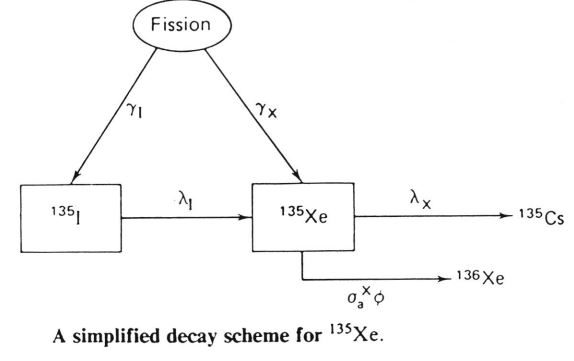
\includegraphics[width=0.7\textwidth]{xenon.jpg}
		\end{figure}\\
		The following ODEs apply:
		\[
		\frac{\partial I}{\partial t} = \Sigma_f \phi \gamma_1 - \lambda_I I
		\]
		\[
		\frac{\partial Xe}{\partial t} = \Sigma_f \phi \gamma_2 + \lambda_I I -\sigma_a^X \phi Xe - \lambda_X Xe
		\]
		At equilibrium,$\frac{\partial Xe}{\partial t} = \frac{\partial I}{\partial t} = 0$ , the iodine and xenon concentrations would be:
		\[
		0= \Sigma_f \phi \gamma_1 - \lambda_I I_\infty
		\]
		\[
		I_\infty= \frac{\Sigma_f \phi \gamma_1}{\lambda_I}  
		\]
		\[
		0 = \Sigma_f \phi \gamma_2 + \lambda_I I_\infty -\sigma_a^X \phi Xe_\infty - \lambda_X Xe_\infty
		\]
		\[
		\sigma_a^X \phi Xe_\infty +\lambda_X Xe_\infty = \Sigma_f \phi \gamma_2 + \lambda_I I_\infty 
		\]
		\[
		Xe_\infty= \frac{\Sigma_f \phi \gamma_2 + \lambda_I I_\infty}{\sigma_a^X \phi + \lambda_X} = \frac{\Sigma_f \phi \gamma_2 + \Sigma_f \phi \gamma_1}{\sigma_a^X \phi + \lambda_X} 
		\]
		\[
		Xe_\infty= \frac{\Sigma_f \phi (\gamma_1+\gamma_2)}{\sigma_a^X \phi + \lambda_X} 
		\]
		After shutdown, the iodine concentration is modeled with the following ODE.
		\[
		\frac{\partial I}{\partial t} = - \lambda_I I
		\]
		\[
		\frac{1}{I}\partial I =  \lambda_I \partial t
		\]
		\[
		I =  I_0 e^{-\lambda_I t}
		\]
		After shutdown, the xenon concentration is modeled with the following ODE.
		\[
		\frac{\partial Xe}{\partial t} = \lambda_I I - \lambda_X Xe
		\]
		\[
		\frac{\partial Xe}{\partial t}+ \lambda_X Xe = \lambda_I I 
		\]
		Multiply by an integrating factor $e^{\lambda_Xt}$
		\[
		\frac{\partial Xe}{\partial t}e^{\lambda_Xt} +\lambda_X Xe e^{\lambda_Xt}= \lambda_I I e^{\lambda_Xt} 
		\]
		\[
		\frac{\partial}{\partial t}Xe e^{\lambda_Xt}= \lambda_I I_0 e^{-\lambda_I t} e^{\lambda_Xt} = \lambda_I I_0 e^{(\lambda_X-\lambda_I )t} 
		\]
		Integrate with respect to $t$ from 0 to t. 
		\[
		Xe e^{\lambda_Xt}-Xe_0= \int_{0}^{t}\lambda_I I_0 e^{(\lambda_X-\lambda_I )t} dt
		\]
		\[
		Xe e^{\lambda_Xt}-Xe_0= \frac{\lambda_I I_0}{\lambda_X-\lambda_I} (e^{(\lambda_X-\lambda_I)t}-1)
		\]
		\[
		Xe =Xe_0 e^{-\lambda_Xt}+ \frac{\lambda_I I_0}{\lambda_X-\lambda_I} \frac{1}{e^{\lambda_Xt}}(e^{(\lambda_X-\lambda_I)t}-1)
		\]
		\[
		Xe =Xe_0 e^{-\lambda_Xt}+ \frac{\lambda_I I_0}{\lambda_X-\lambda_I}(e^{-\lambda_It}-e^{-\lambda_Xt})
		\]
		
		\subsection*{\textbf{Samarium}}
		Assume the following decay scheme for Samarium.
		\begin{figure}[H]\centering
			\includegraphics[width=0.7\textwidth]{Samarium.jpg}
		\end{figure}
		The following ODEs apply:
		\[
		\frac{\partial Pm}{\partial t} = \Sigma_f \phi \gamma_{Pm} - \lambda_{Pm}Pm
		\]
		\[
		\frac{\partial Sm}{\partial t} =  \lambda_{Pm}Pm - \sigma_a^s Sm \phi 
		\]
		Assume constant flux and solve for $Pm$.
		\[
		\frac{\partial Pm}{\partial t} + \lambda_{Pm}Pm = \Sigma_f \phi \gamma_{Pm}  
		\]
		Multiply by an integrating factor $e^{\lambda_{Pm}t}$.
		\[
		\frac{\partial Pm}{\partial t}e^{\lambda_{Pm}t} + \lambda_{Pm}Pme^{\lambda_{Pm}t} =\frac{\partial}{\partial t}Pme^{\lambda_{Pm}t} =\Sigma_f \phi \gamma_{Pm}e^{\lambda_{Pm}t}  
		\]
		Integrate with respect to $t$ from 0 to $t$. 
		\[
		Pm(t)e^{\lambda_{Pm}t} -Pm_0 =\int_{0}^{t}\Sigma_f \phi \gamma_{Pm}e^{\lambda_{Pm}t}dt  
		\]
		\[
		Pm(t)e^{\lambda_{Pm}t} -Pm_0 =\frac{\Sigma_f \phi \gamma_{Pm}}{\lambda_{Pm}}(e^{\lambda_{Pm}t}-1)  
		\]
		\[
		Pm(t) = Pm_0e^{-\lambda_{Pm}t}+\frac{\Sigma_f \phi \gamma_{Pm}}{\lambda_{Pm}}(1-e^{-\lambda_{Pm}t})  
		\]
		Now consider shutdown after steady-state operation long enough to achieve equilibrium. At equilibrium,$\frac{\partial Pm}{\partial t} = \frac{\partial Sm}{\partial t} = 0$ , the concentrations would be:
		\[
		0 = \Sigma_f \phi \gamma_{Pm} - \lambda_{Pm}Pm_\infty
		\]
		\[
		Pm_\infty = \frac{\Sigma_f \phi \gamma_{Pm}}{\lambda_{Pm}}
		\]
		\[
		0 =  \lambda_{Pm}Pm_\infty - \sigma_a^s Sm_\infty \phi 
		\]
		\[
		Sm_\infty =  \frac{\lambda_{Pm}Pm_\infty}{\sigma_a^s\phi} 
		\]
		\[
		Sm_\infty =  \frac{\lambda_{Pm}}{\sigma_a^s\phi}\frac{\Sigma_f \phi \gamma_{Pm}}{\lambda_{Pm}} 
		\]
		\[
		Sm_\infty = \frac{\Sigma_f \gamma_{Pm}}{\sigma_a^s}
		\]
		After shutdown:
		\[
		\frac{\partial Pm}{\partial t} = -\lambda_{Pm} Pm
		\]
		\[
		Pm = Pm_\infty e^{-\lambda_{Pm} Pm}
		\]
		\[
		\frac{\partial Sm}{\partial t} = \lambda_{Pm} Pm
		\]
		\[
		\frac{\partial Sm}{\partial t} = \lambda_{Pm} Pm_\infty e^{-\lambda_{Pm} Pm}
		\]
		Integrate with respect to $t$ from 0 to $t$.
		\[
		Sm(t)-Sm_\infty = \int_{0}^{t}\lambda_{Pm} Pm_\infty e^{-\lambda_{Pm} Pm}dt= \frac{\lambda_{Pm} Pm_\infty}{-\lambda_{Pm}}(e^{-\lambda_{Pm} Pm}-1 )
		\]
		\[
		Sm(t)=Sm_\infty+ Pm_\infty(1-e^{-\lambda_{Pm} Pm})
		\]
		\subsubsection*{Equilibrium Reactivity Worth: Xenon}
		\[
		\Delta \rho = \frac{-\Sigma_a}{\nu\Sigma_f} = \frac{-\sigma_a}{\nu\Sigma_f} Xe_\infty = \frac{-\sigma_a}{\nu\Sigma_f} \frac{\Sigma_f\phi(\gamma_1+\gamma_2)}{\lambda_{Xe}+\sigma_a^Xe \phi} = \frac{-\sigma_a\phi(\gamma_1+\gamma_2)}{\nu(\lambda_{Xe}+\sigma_a^{Xe}\phi)}
		\]
		\[
		\Delta \rho = \frac{-\phi(\gamma_1+\gamma_2)}{\nu(\frac{\lambda_{Xe}}{\sigma_a^{Xe}}+\phi)} 
		\]
		For large fluxes $\phi >> \frac{\lambda_{Xe}}{\sigma_a^{Xe}}$
		\[
		\Delta \rho = \frac{-\phi(\gamma_1+\gamma_2)}{\nu\phi)} = \frac{-(\gamma_1+\gamma_2)}{\nu)} \approx -0.026  
		\]
		\subsubsection*{Equilibrium Reactivity Worth: Samarium}
		\[
		\Delta \rho = \frac{-\Sigma_a}{\nu\Sigma_f} = \frac{-\sigma_a}{\nu\Sigma_f} Sm_\infty 
		\]
		From earlier $Sm_\infty = \frac{\Sigma_f \gamma_{Pm}}{\sigma_a}$ 
		\[
		\Delta \rho = \frac{-\Sigma_a}{\nu\Sigma_f} = \frac{-\sigma_a}{\nu\Sigma_f} \frac{\Sigma_f \gamma_{Pm}}{\sigma_a} = \frac{-\gamma_{Pm}}{\nu}\approx0.00463 
		\]
			
\end{document}